\documentclass[letterpaper,twocolumn,10pt]{article}
\usepackage{usenix,epsfig,endnotes,graphicx,url}
\begin{document}

%don't want date printed
\date{}

%make title bold and 14 pt font (Latex default is non-bold, 16 pt)
\title{\Large \bf Cyclone: Replication Middleware for NVM Applications}

%for single author (just remove % characters)
%\author{
%  {\rm Paper #: XXX }\\
%  XXX
%  \and
%  {\rm YYY}\\
%  YYY
%} % end author

\maketitle

% Use the following at camera-ready time to suppress page numbers.
% Comment it out when you first submit the paper for review.
%\thispagestyle{empty}

\subsection*{Abstract}
The introduction of non-volatile directly attached memory in datacenters - in
the form of NVDIMMs and new memory technologies allows efficient data structures
to be built on non-volatile heaps that provide good performance coupled with
durability. However high availability remains a problem for these primarily
single machine solutions. While transactional interfaces built over RDMA capable
networking hardware offer a viable alternative, such hardware is often
unavailable in datacenters. Cyclone offers a solution to this problem by
providing transparent replication middleware that can be used with Intel's Non
Volatile Memory Library (NVML) to construct durable data-structures that map
keys to values.  Cyclone is designed around an optimized userspace networking
stack to reduce latency and can scale its consensus protocol across cores and
network ports to provide good throughput under load. We show that Cyclone can
replicate as many as 7 million updates a second using just 4 commodity 10 GigE
ports on a machine.

\section{Introduction}
Memory technology in datacenters is due to undergo a paradigm shift with the
increased use of directly addressable non-volatile memory both in the form of
battery backed non-volatile DIMMs~\cite{farm} as well as newer memory types
such as 3D XPoint~\cite{pmfs, bpfs}. In anticipation, libraries that allow
programmers to build durable data structures on non-volatile heaps have become
available~\cite{mnemosyne, nvheaps, cdds}  - an example of such a
library that we have used in this paper is Intel's non volatile memory library
(NVML)~\cite{nvml}. A missing piece however is a component to make such durable 
data structures highly available using replication across a commodity network
such as ethernet. Existing solutions that offer good performance are biased
towards pure transactions across RDMA with a dependence on external services
(such as zookeeper~\cite{zookeeper}) and application specific code for
fault recovery~\cite{farm, htm}.
This is a problem for programmers using NVML to construct durable and available 
data structures where one cannot apriori guarantee the availability of
RDMA (for e.g., when running on externally hosted environments or public
clouds).

Cyclone is prototype replication middleware that aims to demonstrate that one
can add fault tolerance transparently to a specific class of client server
applications written on top of libraries such as NVML. We specifically target
key-value maps in this paper and in that context make two key
contributions. First, we propose a simple API that enables server state to be
replicated without the programmer needing to worry about fault recovery. This
allows one to start by building a concurrent durable data structure using
libraries such as NVML and add availability at a later stage using Cyclone. The
second contribution is to show that one can achieve reasonably good replication 
performance using commodity ethernet via innovations in the networking stack and
by scaling replication with the application. This result should be a useful
design point for developers looking to deploy applications on non-volatile heaps
in commodity ethernet-based environments such as public clouds.

\section{Single Node Programming Model}
Cyclone assumes a concurrent durable application on a non-volatile heap as the
starting point. A number of libraries and filesystems make this possible
today~\cite{nvml, dax, pmfs, mnemosyne, nvheaps, cdds}. Cyclone currently
supports applications built on top of Intel's Non Volatile Memory Library
(NVML~\cite{nvml}). We describe NVML's programming model in this section to
provide adequate background for the rest of this paper. NVML requires 
that code that makes changes to the non-volatile heap is enclosed in a crash
consistent transaction such that either all of the transaction executes or none
of it executes in the event of power failures.
%This is critical to maintaining consistency as the data structure, being
%durable, must survive across power failures.
Figure~\ref{fig:example} illustrates the use of NVML to build a persistent
linked list. Updates to the linked list are enclosed in a NVML transaction to
avoid corruption due to power failure. It is also worth noting that NVM
libraries such as NVML usually allow remapping non-volatile heaps to a different
virtual memory address range across restarts (e.g., using {\tt TOID} macros to
implement fat pointers in NVML).

\begin{figure}
  { \scriptsize
\begin{verbatim}
struct ll_node {
  int value;
  TOID(ll_node) next;
};

void insert_after(TOID(ll_node) prev, 
                  TOID(ll_node) new_node)
{
  TX_BEGIN {
    TX_ADD(new_node);
    D_RW(new_node)->next = D_RO(prev)->next;
    TX_ADD(prev);
    D_RW(prev)->next = new_node;
  } TX_END
}

\end{verbatim}
  }
\caption{A Persistent Linked List}
\label{fig:example}
\end{figure}

It is easy to turn the linked list example in NVML into a concurrent linked list
by simply adding a lock to it. Such a lock can be maintined in volatile DRAM if
so desired for performance. More sophisticated fine-grained or optimistic
concurrency control mechanisms for NVM are also
possible~\cite{mnemosyne, cdds, nvheaps}.

\section{Replication}
Cyclone is designed to add fault tolerance to NVML client server applications
via replication -- a quorum of machines maintains \emph{equivalent} state.
Server state is queried and manipulated via RPC calls from clients.
Cyclone replicates the RPC call itself across replicas rather than replicating
every access (to the server state) made during execution of the RPC call.

Cyclone provides strongly consistent replication - every machine in the quorum
of replicas maintains a log of RPC calls. Cyclone treats the RPC call itself as
a variable sized opaque blob of data, leaving the application free to choose how
it wishes to marshall call related details and arguments. All machines agree on
the committed sequence of RPC calls in the log. We achieve this by running an
instance of the RAFT~\cite{raft} consensus protocol to keep the log of RPC calls
on different machines in synchronization. Specially flagged `read-only` RPC
calls are executed only on the leader replica and are not replicated.

\subsection{Decoupled Replication}
\label{sec:decouple}
The standard replicated state machine approach requires that commands (entries
in the log) be committed before they can be applied to the state machine --
i.e. in our case before the RPC call can be executed. In contrast, Cyclone
decouples execution of an RPC call on any replica from its replication.
The fact that RPC calls that modify state must themselves be executed
in a crash consistent transaction allows us to overlap execution with
replication. Normally, this would be a problem as replication might fail for a
number of reasons but primarily due to change of leadership and subsequent
rollback of previously appended (but not committed) log entries. To solve this
problem, Cyclone delays the actual commit of the failure atomic transaction
until after the replication is complete. In the event that replication fails,
the transaction is aborted and any changes to the non volatile heap are rolled
back. Figure~\ref{fig:async_rep} shows a pseudocode description of how the
runtime handles \emph{decoupled replication}.

\begin{figure}
{ \scriptsize
\begin{verbatim}
Initiate replication of RPC call and arguments 
TX_BEGIN { 
  Execute RPC call and modify local NVM 
  Block till replication result known 
  if(replication failed) {
     TX_ABORT 
  } 
} TX_END
\end{verbatim}
}
\caption{Decoupled Replication}
\label{fig:async_rep}
\end{figure}

Decoupled replication provides good performance and we believe it would be
the common case for RPC calls replicated via Cyclone. However the program might 
on occasion require successful replication to be a precondition to exection.
A case where we find this necessary is
\textit{output commit}~\cite{output_commit} - where the RPC call has
external side effects (e.g., communication with other machines in the cluster)
and therefore crash consistency is insufficient to roll back the execution of
the RPC call in the event that replication fails. We therefore provide users the
ability to declare at the client side that an RPC call should execute
in a coupled manner at the server side. Cyclone would then ensure that the RPC
call is successfully replicated before it attempts execution on any of the
replicas.

\subsection{Network Stack}
Cyclone is designed around DPDK~\cite{dpdk} -- a high performance network stack
optimized for Intel processors. DPDK provides convenient access to packets
arriving at an ethernet NIC by moving them into packet buffers and directly
placing those buffers into the last level cache of the CPU during DMA~\cite{ddio}.

Cyclone separates the available CPU cores on a machine, in a configurable way,
into cores dedicated to work related to the (RAFT) consensus protocol and cores
decidated to running application code. Each RAFT core runs an \emph{independent}
instance of the RAFT protocol. RAFT cores pass work to the application cores
through lock-free double ended queues. A RAFT core dispatches an incoming RPC
call for execution simultaneously with sending it out for replication.

Each RAFT core has a dedicated NIC queue pair. The input queue receives RPC
calls from clients as well as RAFT protocol related traffic. The output queue
only carries RAFT protocol related traffic. Each application core has a
dedicated \emph{output} queue on the NIC. When completed, the response to the
RPC call is sent from the application core via its dedicated output queue. This
division of NIC queues eliminates the need for synchronization between RAFT
cores and application cores when accessing the NIC.

In the event that the machine has multiple NICs, Cyclone spreads the network
demands and scales by binding each RAFT or application core to a specific NIC
and picking the necessary queues from that NIC.

\subsection{Zero Copy Batching}
Consensus protcols such as RAFT usually have a simple common case path. Once a
quorum leader is elected, the leader's primary job is to transmit new entries
appended to its persistent log to its followers. The primary job of a follower
is to receive these entries, append them to its persistent log and send
acknowledgments to the leader. An entry is considered committed when the leader
receives an acknowledgment for an entry from a majority of the quorum. Followers
receive intimation of committed entries as piggybacked information on subsequent
replication messages. The common case path at the leader lends itself to zero
copy since the same set of log entries is sent to all replicas.

In order to avoid an additional copy of the incoming RPC call contents from DRAM
to persistent memory, Cyclone allocates space for packet buffers on the non-volatile
heap. However, since packet data is cached, Cyclone ensures durability
(or persistence) of this data by explicitly flushing the dirty
cachelines~\cite{pmfs}. Cyclone maintains its log as a circular sequence of
pointers to packet buffers and therefore the append operation is completed by
adding a pointer to the received packet and flushing the cacheline containing
the pointer.

We exploit the fact that DPDK allows prepending data to a packet
without physically moving the data in a packet buffer. The received packet
contains only the RPC call from the client. We prepend a RAFT related header
(containing the previous log index, previous log term, leader's term and
leader's commit point~\cite{raft}) to the packet buffer itself. To this RAFT header 
we then prepend an IPv4 header. We assign pre-determined values to the
IP address fields in order to exploit 5-tuple steering at the receiving NIC for 
the placement of the incoming packet in the correct queue.
This composite packet buffer is then sent \emph{unchanged} to every replica.
To properly route the packet through switches, for each follower replica we
allocate a small buffer containing an ethernet header with appropriate addresses
and \emph{chain} the buffer in front of the prepared packet - thereby ensuring
that we do not need to change the contents of the packet itself.

Although the common case path in RAFT is straightforward, it still requires
hundreds of cycles (or a few microseconds) to process each log entry, which is
a significant amount in the face of sub 10 us network latency between nodes with
DPDK. We amortize this overhead when operating under load by
batching multiple RPC calls together and treating the batch as a single RAFT log
entry.  DPDK by itself can efficiently batch incoming packets under load,
therefore allowing the user to easily receive a burst of packets
(currently limited to 32) rather than a single packet for a polling call.
DPDK further allows chaining packet
buffers together and treating the chain as a single packet. This is convenient
for our zero copy approach and we chain packet mbufs together to form a single
packet. Since the entire chain is sent as a single packet when being replicated,
the length of a chain is limited by the size of the coalesced packet, that must
fit into an ethernet jumbo frame of approximately 9KB.

\begin{figure}
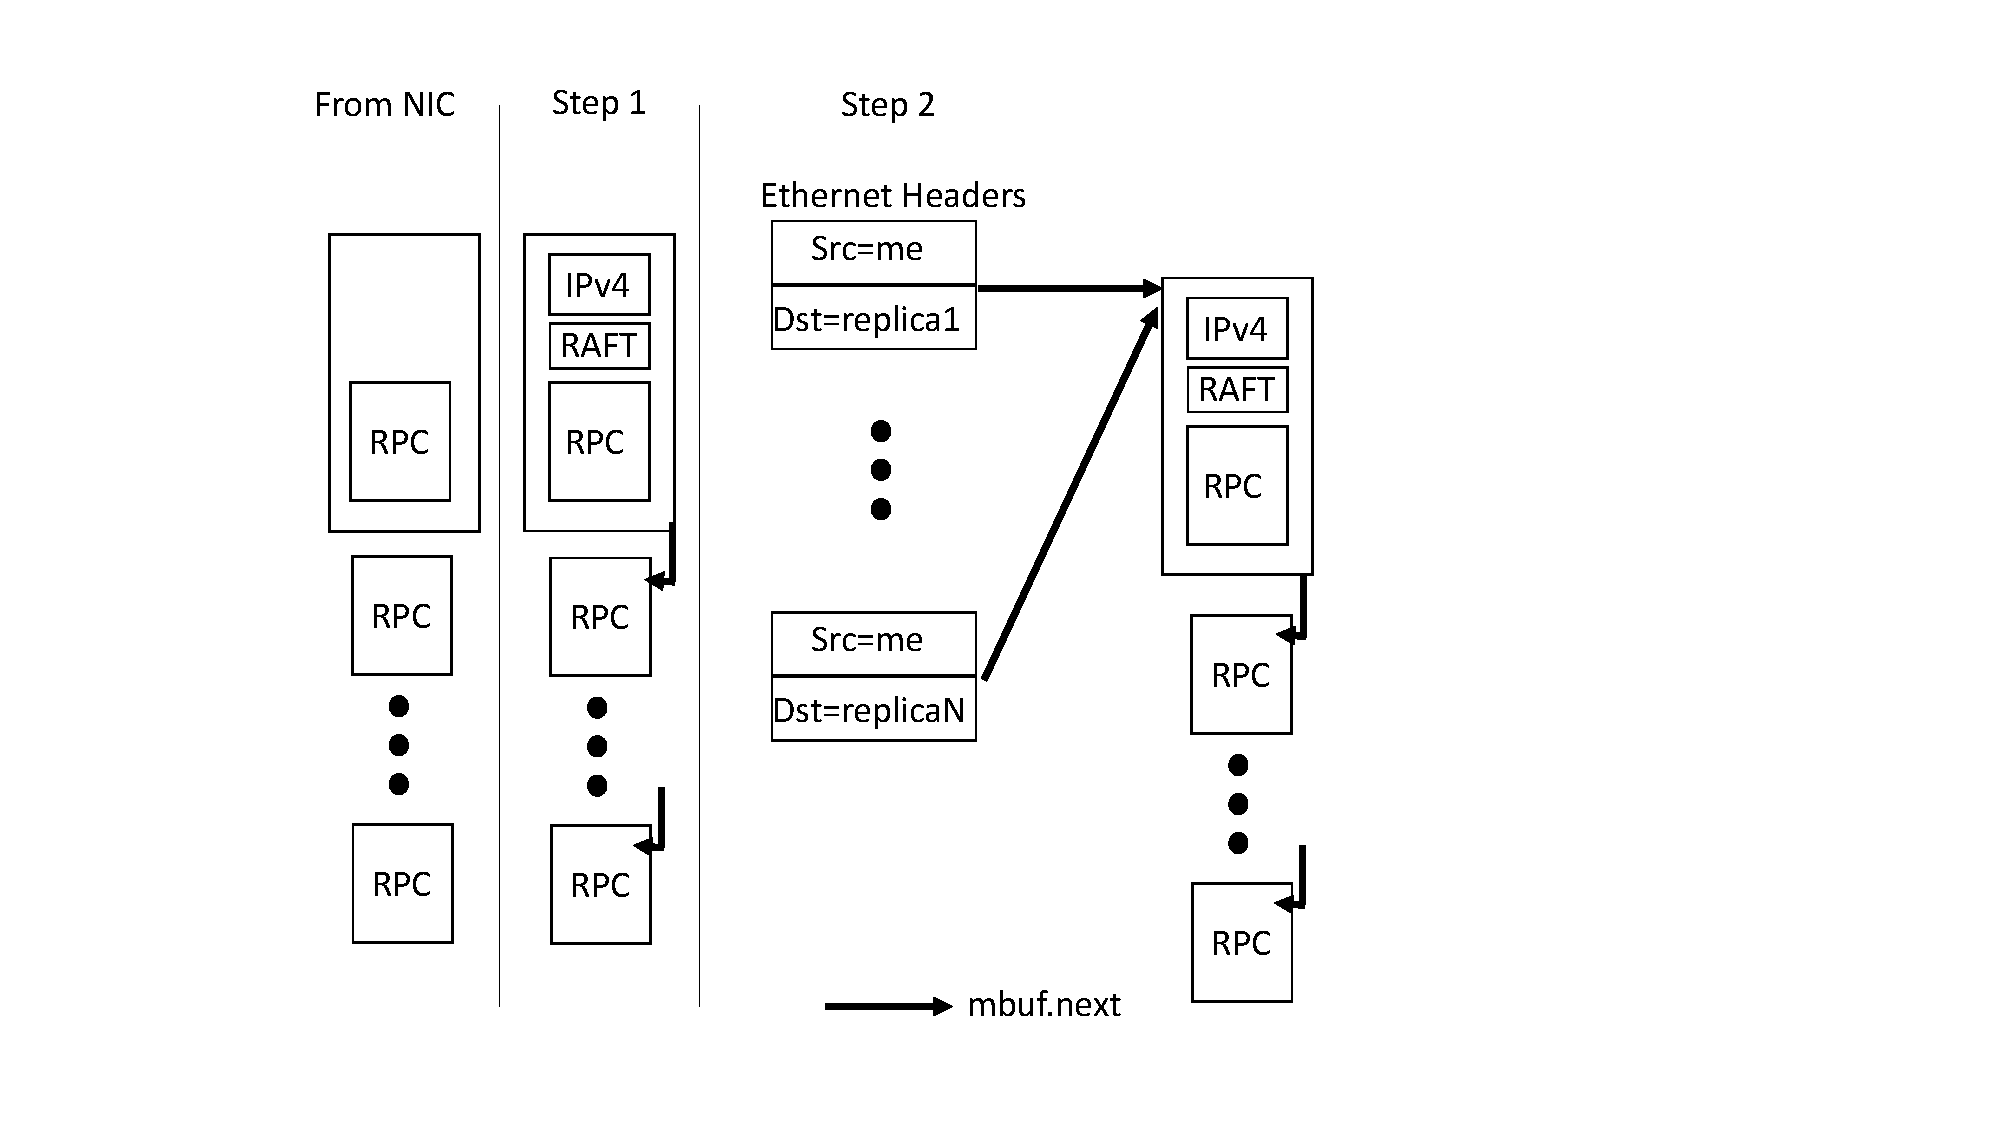
\includegraphics[width=0.7\textwidth,height=6cm]{figures/chain.pdf}
\caption{Zero Copy Batching}
\label{fig:zc_batch}
\end{figure}

This set of transformations to incoming request packets from clients at the
leader replica is summarized in Figure~\ref{fig:zc_batch}. 

\subsection{RPC Call Execution}
\label{sec:exec}
We now describe how RPC calls are executed and results returned to the
client. There are two important aspects of RPC call execution in Cyclone -
steering and at most once semantics.

An RPC call via Cyclone must traverse a specific RAFT core (and associated
consensus protocol instance) and specific application core. These details are
provided by the user when making the RPC call to the client side library
provided by Cyclone. The user therefore is aware of the number of execution
cores and RAFT instances and given complete control of \emph{RPC call steering}.
For most applications we envisage a simple modulo hashing scheme should suffice
for load balancing.

Cyclone provides at most once semantics. It supports a large but fixed (at
startup time) number of clients. Each RPC call from a client bears the client
number and a sequence number. \emph{Each execution core independently enforces
  that accepted RPC calls from the same client bear increasing sequence
  numbers}. This is done by storing the last executed sequence number for every
client in a per-core durable datastructure as part of the crash consistent
transaction wrapping the execution of the RPC call. Even in the presence of
fail-overs, this durable memory of sequence numbers seen from a client ensures
at most once semantics. In addition to guarding against repeated execution of
the same call, Cyclone also remembers the \emph{result} of the last executed RPC
call from every client. This is done to assist clients (particularly stateless
clients). Cyclone allows the client to query the last seen sequence number and
result for that RPC call from the quorum of servers.

\section{A Durable Replicated Hash Table}
\label{sec:example}
We now demonstrate how Cyclone can be used in practice by putting together an
example of a linearizable hash table - a useful and common data structure.
The baseline is a durable hash table written in NVML that runs on a
single machine in client-server mode. The server side maintains the durable
open-addressed hash table and services client RPC calls to insert and delete
key-value pairs and lookup keys.

A durable hash table is simple to derive from a volatile hash table and readily
available in NVML as an example~\cite{nvml_hash}. To use that (non client-server)
example with Cyclone we added a simple RPC call format, manually marshalled and
demarshalled the few arguments to the RPC call in an RPC call handler we wrote -
a few tens of lines of code. Finally, we added a simple client driver program (a
few tens of additional lines of code).

In order to use the hash table with Cyclone, we simply need to to declare the
RPC call handler as the point of entry to Cyclone at the server end.  The client
end issues RPC calls via Cyclone's client side library. Crucially neither side
involves fault awareness or fault recovery code - a key goal for Cyclone.

There are two interesting challenges in scaling the performance and improving
the utility of the linearizable and durable hash table. The first is to ensure
linearizability while scaling performance by adding RAFT cores and application
cores. The second is to support distributed transactions - that manipulate a set
of key-value pairs atomically in the face of failure.

\subsection{Scaling}
Scaling the performance of the hash table by using multiple RAFT cores and
application cores presents determinism related challenges. Two RPC calls being
steered through different RAFT cores can end up executing in different orders on
different replicas even if steered to the same application core. At the same time,
two RPC calls steered through the same RAFT core but dispatched to different
application cores can end up completing in different orders on different replicas.

Our solution to this problem in Cyclone is to observe that replicas of the hash
table require \emph{per-key determinism} and not determinism across \emph{all}
operations. We therefore steer operations to the same key to the same RAFT core
and the same application core, by hashing the key to determine the RAFT core and
execution core. The actual configuration of the hash table therefore can be
different across different replicas - for example due to the insertion of two
keys mapping to the same hash bucket completing in different orders across
different replicas. However, since the results of insert, delete and lookup
operations for a key depend only on previous operations to the same key the
replicas provide identical results for committed operations.

The RPC call steering mechanism described above leaves the programmer free to
use any synchronization mechanism they wish between concurrent accesses from the
application cores to the data structure, since the ordering between accesses
from different cores is allowed to be non-deterministic. For our open addressed
hash table we chose the simple scheme of a per-bucket lock.

\subsection{Distributed Transactions}
A useful primitive for many distributed systems is the ability to run
distributed transactions - an atomic sequence of conditional updates spanning
multiple groups of replicas. Distributed transactions have two distinct facets:
atomicity and fault tolerance. Distributed transactions appear atomic with
respect to other atomic transactions and simple updates or reads by virtue of
standard concurrency control techniques. A common technique is strict two phase
locking: acquire all locks, update the locked objects and finally release all
the locks. We believe that NVM application programmers - particularly those
having experience with concurrent code should not find it hard to deal with
distributed concurrency. The hard part for most programmers is likely to be the
second aspect: fault tolerance. A distributed transaction spans many machines
and has a large footprint to clean up in the event of failure. Failure handling
is made more complex when considering cascading failures - further failures
while recovering from a failure. Cyclone was designed to allow primitives such
as distributed transctions to be added without the programmer needing to worry
about faults or write fault recovery code. As an exercise we show how to add
support for distributed transactions to our hash table.

We support distributed transactions in our hash table by allowing the user to
specify a group of insert/delete/lookup operations that must occur
atomically. We use the existing bucket locks to support a simple two phase
locking protocol to implement the transction. A client makes an RPC call to the
server specifying the transaction and the server executes it on the client's
behalf. Execution of the transaction has four distinct phases: acquire locks,
verify values, apply updates and finally release locks.

We guard against faults by executing the the entire transaction on a quorum of
machines via Cyclone. All machines in the quorum execute the transaction, making
calls to other quorums to execute steps in the two phase locking protocol. Since
execution of the RPC call leaves \emph{externally visible side effects} by
virtue of the RPC calls it makes we require output
commit~\cite{output_commit}. This is achieved if the execution is guaranteed to
complete once it starts. This is simply achieved by a flag in the RPC call that
turns off decoupled execution (Section~\ref{sec:decouple}). The flag causes
execution to start only after the RPC call has been successfully replicated.

Next, we need to ensure that although every machine in the quorum makes all
necessary RPC calls, the call itself is executed only once. This is achieved by
using Cyclone's at most once semantics. All machines in the quorum executing the
transaction use the same client identifier and the same montonically increasing
sequence of RPC call numbers. Finally, we need to deal with the fact that
Cyclone only remembers the last executed RPC call for a client. This means that
if different machines in the quorum move at different speeds, some machines will
not receive a response to the RPC call - they will instead receive an error that
tells them that they are too far behind.

To ensure that the transaction is still guaranteed to complete, we use a
\emph{different} client identifier for each phase. Thus, until the transaction
completes and a new one is started the response for any RPC call continues to be
available. Figure~\ref{fig:dist_tx} shows in pseudocode the server side details
of a transaction. One initiated, the distributed transaction is guaranteed to
complete given quorum availabilty. However, if the client requires intimation of
completion, the final transaction state can be written to a distinguished
partition as part of the transaction itself.

We note that this design is not intended for performance, under the assumption
that distributed transactions will be infrequent compared to single key
operations.  On the other hand, it is worth comparing the lack of any need for
explicit fault recovery in Cyclone with fault recovery in systems systems that
explicity require such cleanup (~\cite{farm}, pp 59--63).  We believe that
such designs, which make availability easy for NVM applications are key to
increasing the adoption rate of NVM by datacenter operators.

\begin{figure}
{ \scriptsize
\begin{verbatim}
wait until RPC call is replicated
respond to client saying tx accepted for execution
acquire:
 set client identifier to 1
 for each machine
   Acquire write or read locks on the machine
   If machine reponds RPC sequence too old
     Transaction completed by someone else

update:
 set client identifier to 2
 for each machine
   Update object
   If machine reponds RPC sequence too old
     Transaction completed by someone else
 
release:
 set client identifier to 3
 for each machine
   Update object
   If machine reponds RPC sequence too old
     Transaction completed by someone else

optional:
 write transaction result to <quorum_tx_result>
\end{verbatim}
}
\caption{Distributed Transactions}
\label{fig:dist_tx}
\end{figure}

\section{Evaluation}
We evaluate Cyclone against its design goals by using it for up to 3-way
replication in a cluster of twelve 48 core Xeon servers. Three servers run
Cyclone's server side code, while the remaining machines run multithreaded
clients. The server side machines are each
equipped with four commodity 82599-based 10 Gbit ethernet ports, while each
client machine has one 82599-based 10 Gbit ethernet port. All the machines are
connected through the same 10 Gbit switch. We use 8 cores on the
server machines for running 8 instance of RAFT, leaving 39 cores to run
application code. The last remaining core is reserved for management code. We
use NVML with the non volatile pool held in DRAM, which proxies for the
performance we would expect from NVDIMMs. We evaluate Cyclone in three stages.

First, we evaluate pure replication performance by replicating RPC
calls. Cyclone simply replicates the contents of the RPC call without executing
it and returns a response to the client when replication is complete.
Figure~\ref{fig:pure_rep} shows the results. We consider two cases, one where
the clients send an RPC call with no payload and one where they add a 512 byte
dummy payload. For the no payload case the bottleneck is the message handling
rate. We note that Cyclone can handle small message replication rates as high as
\emph{7 million messages a second}. In the case of RPC calls with 512 byte
payloads, the bottleneck is the available network bandwidth. To show this, we
also plot transmit throughput derived from the message by adding the rate at
which data is sent to replicas from all the 8 quorum leaders to the rate at
which responses are sent back to the clients.  It is interesting to note that
with 3 replicas Cyclone achieves \emph{more than 40 Gbps} of bandwidth. The
reason for this is that the quorum leaders can end up residing on different
machines. Although replication traffic is still limited by the receive bandwidth
at follower replicas, the responses to the clients, originating from different
machines have access to independent 4x10GigE ports, allowing total transmit
throughput to exceed 40 Gbps. Although not discussed in this paper, Cyclone's
control plane is designed to exploit this by trying to spread quorum leaders
across machines.

Also worth noting is that thanks to DPDK's low latency access to the NICs, three
way replication costs as little as 25 us of latency in the unloaded case. This
latency is measured at the client and therefore is four commodity 10 GigE
network hops through the switch, with each hop taking under 7 us including
network stack delays. These results should serve to illustrate that simple
commodity ethernet can indeed provide reasonable replication performance with a
carefully designed software stack that can exploit it.

\begin{figure}
\begin{tabular}{cc}
\begin{minipage}{0.25\textwidth}
  \hspace{-0.17in}
  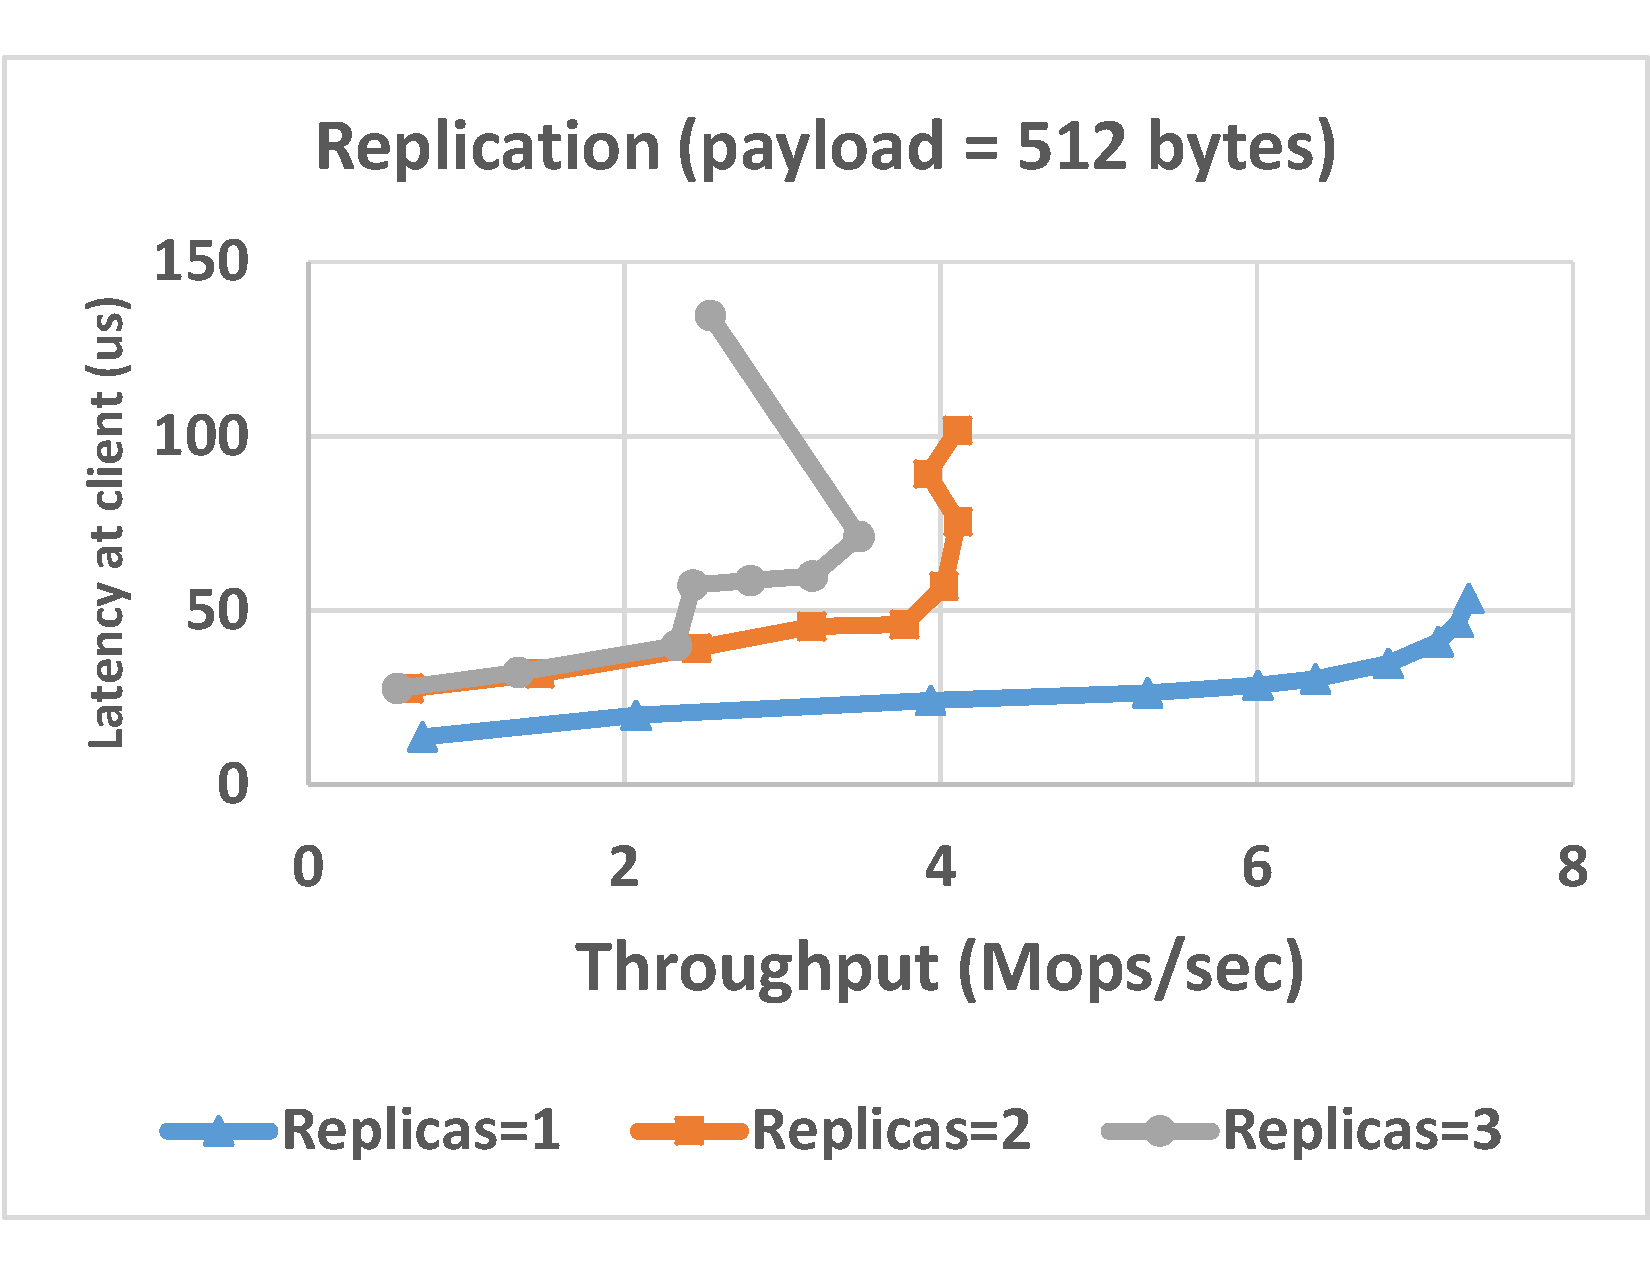
\includegraphics[width=\textwidth,height=3cm]{results/replication_mops_0.pdf}
\end{minipage}&
\begin{minipage}{0.25\textwidth}
  \hspace{-0.37in}
  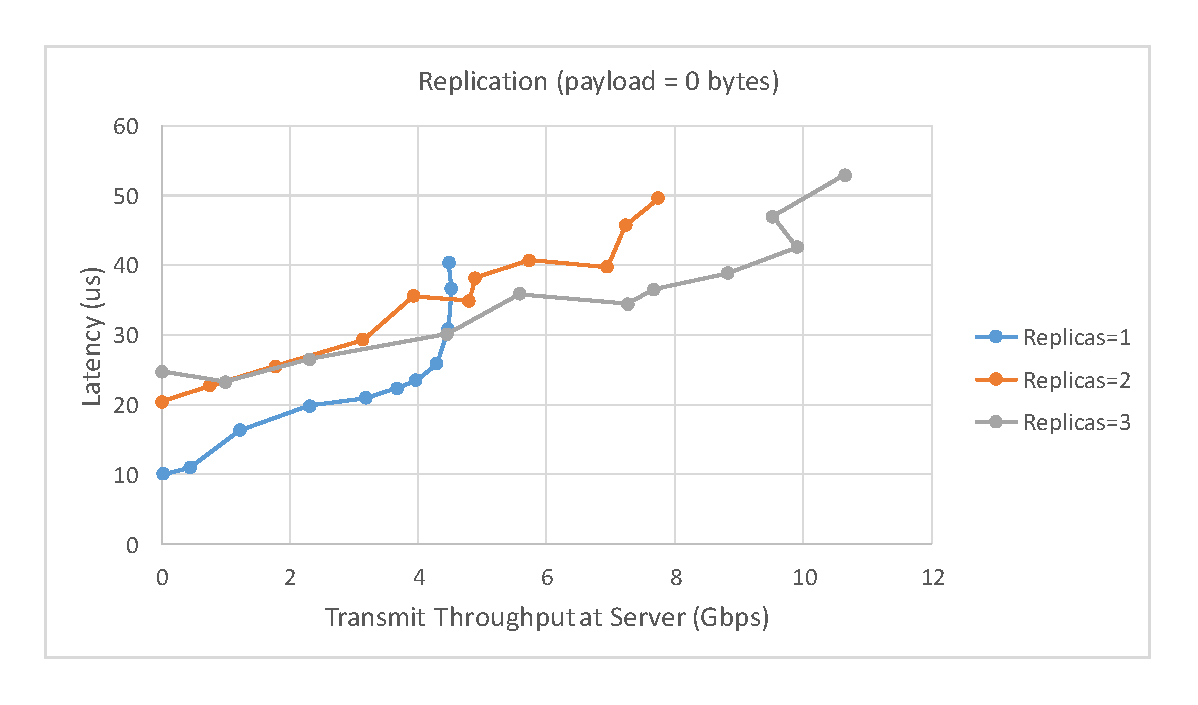
\includegraphics[width=\textwidth,height=3cm]{results/replication_gbps_0.pdf}
\end{minipage}\\
\begin{minipage}{0.25\textwidth}
  \hspace{-0.17in}
  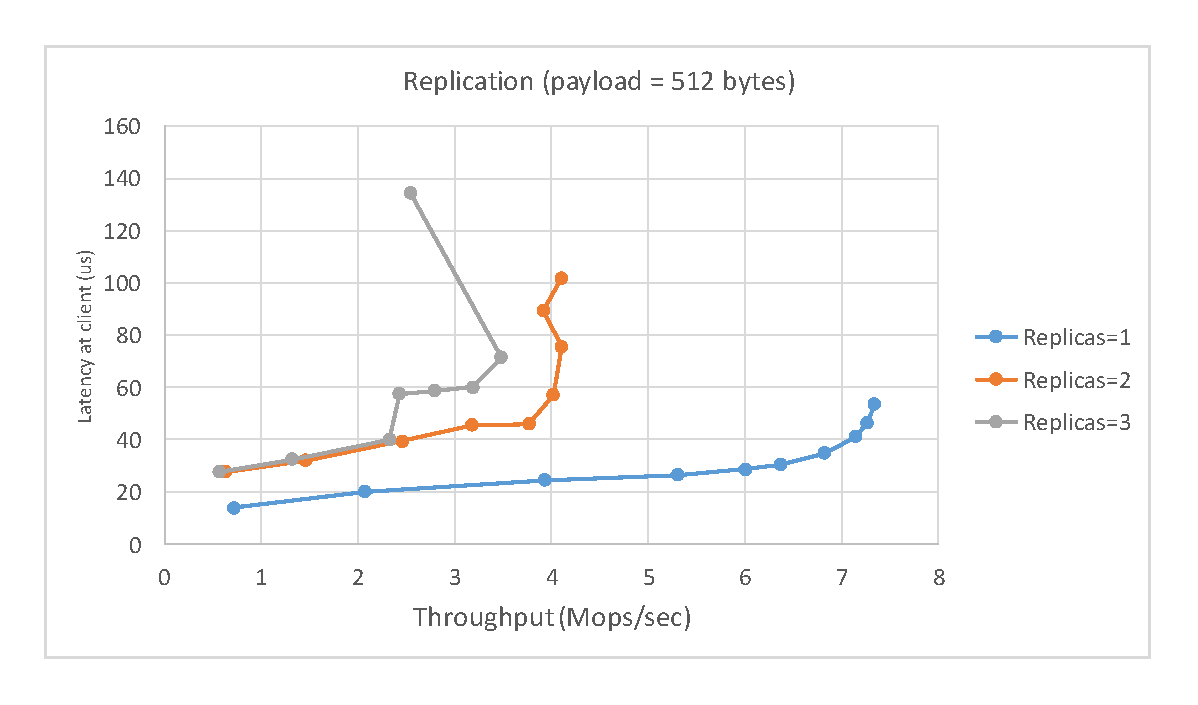
\includegraphics[width=\textwidth,height=3cm]{results/replication_mops_512.pdf}
\end{minipage}&
\begin{minipage}{0.25\textwidth}
  \hspace{-0.37in}
  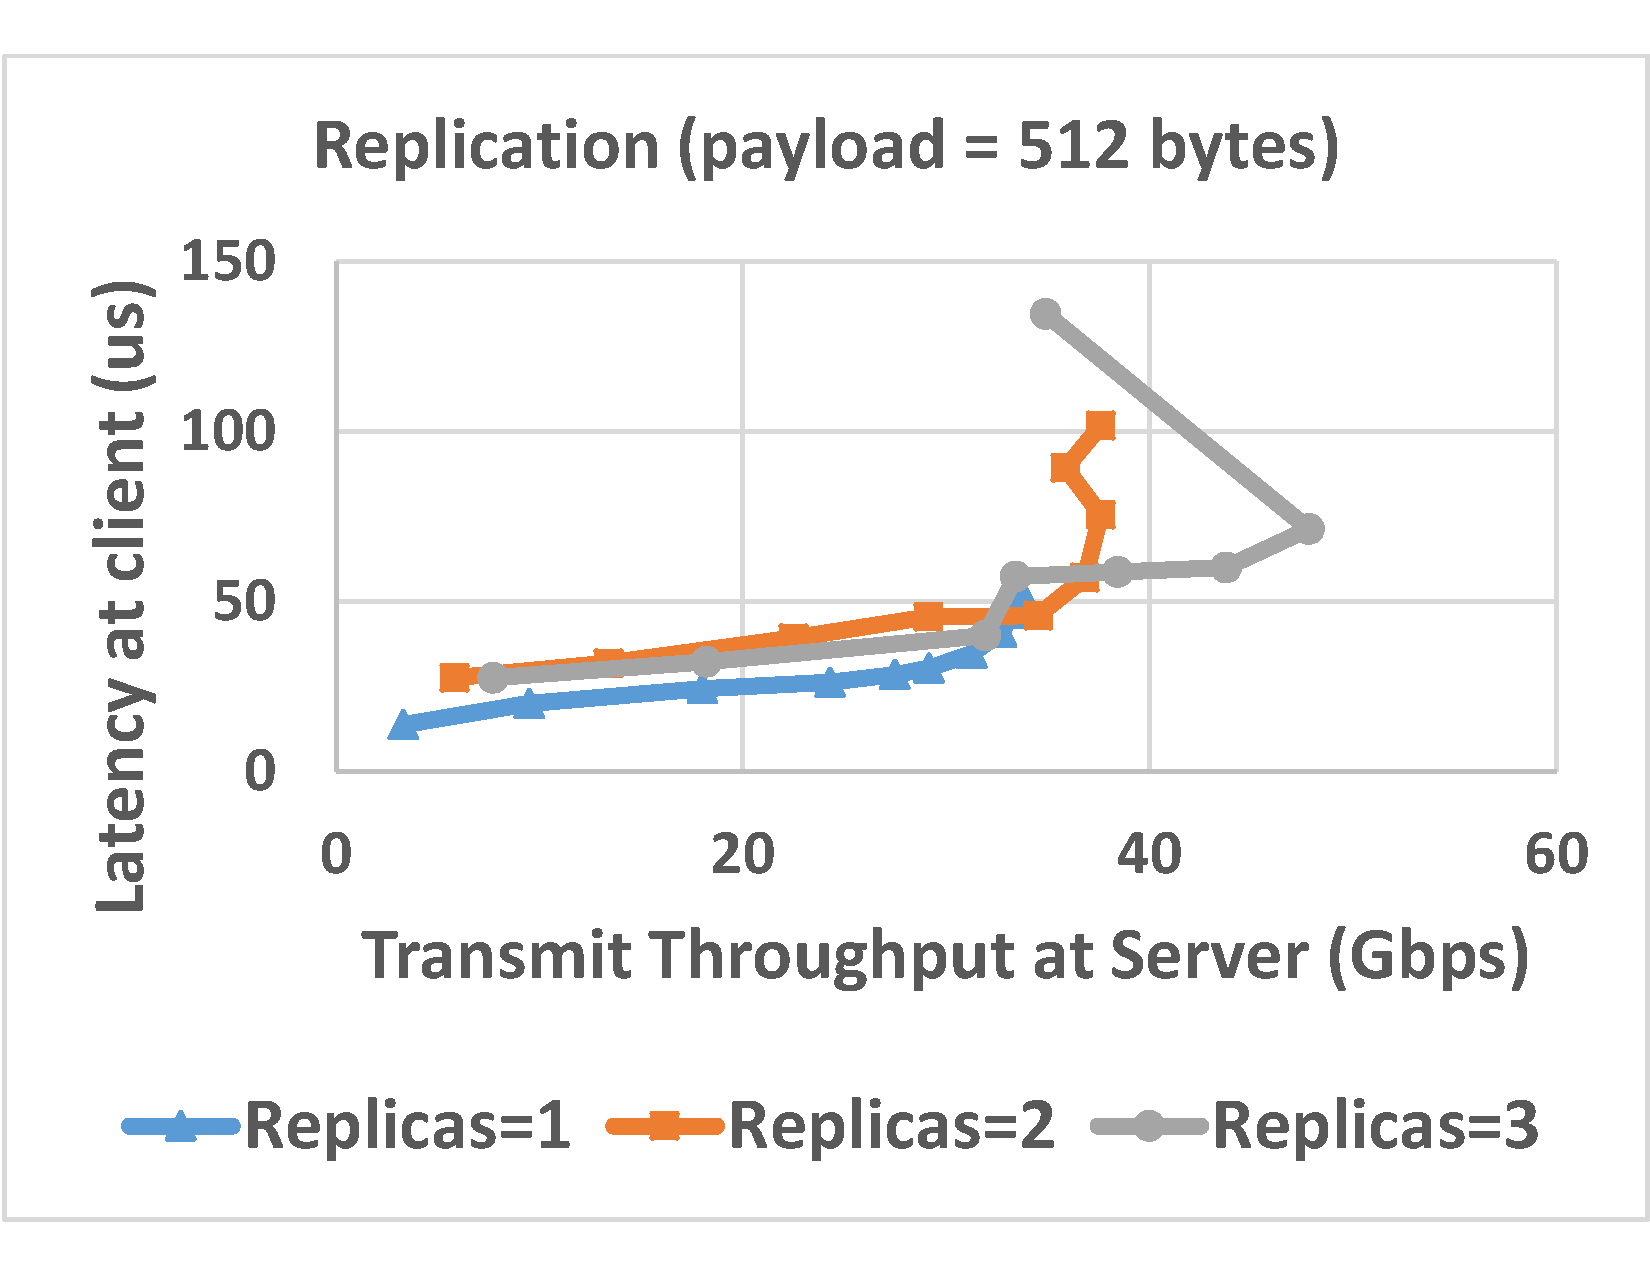
\includegraphics[width=\textwidth,height=3cm]{results/replication_gbps_512.pdf}
\end{minipage}
\end{tabular}
\caption{Pure Replication}
\label{fig:pure_rep}
\end{figure}

Next, Figure~\ref{fig:cc_rep} shows the effect of adding a crash
consistent transaction where the application still does nothing but Cyclone
durably remembers the last sequence number and RPC call result (the application
simply returns the received payload). Throughput is now bottlenecked by NVML
allocator performance at just under a million messages a second. The final
result is adding the hash table in the picture with the clients updating the
values of keys already present in the hash table - a stable workload for easy
comparison. As Figure~\ref{fig:app_rep} shows performance stays at the just
under 1M calls a second mark for pure updates. We also show a
pure read only case where the clients only query the value of a key - there is
no replication \emph{nor} any crash consistent transaction applied. It is
interesting to note that the pure read only case is bottlenecked almost at the same
point as the pure replication case of 7 million operations a second.

These results lead us to conclude that Cyclone provides adequate performance
headroom for transparent replication in NVML applications. In fact our current
focus in the light of these results is towards improving application performance
on top of NVML rather than improving the performane of replication in Cyclone.
%NVML is a general purpose library written for a variety of
%substrates including traditional SSD based storage and there is adequate room
%for improvement of performance for applications running on directly attached
%persistent memory with close to DRAM performance.

\begin{figure}
\begin{tabular}{cc}
\begin{minipage}{0.25\textwidth}
  \hspace{-0.17in}
  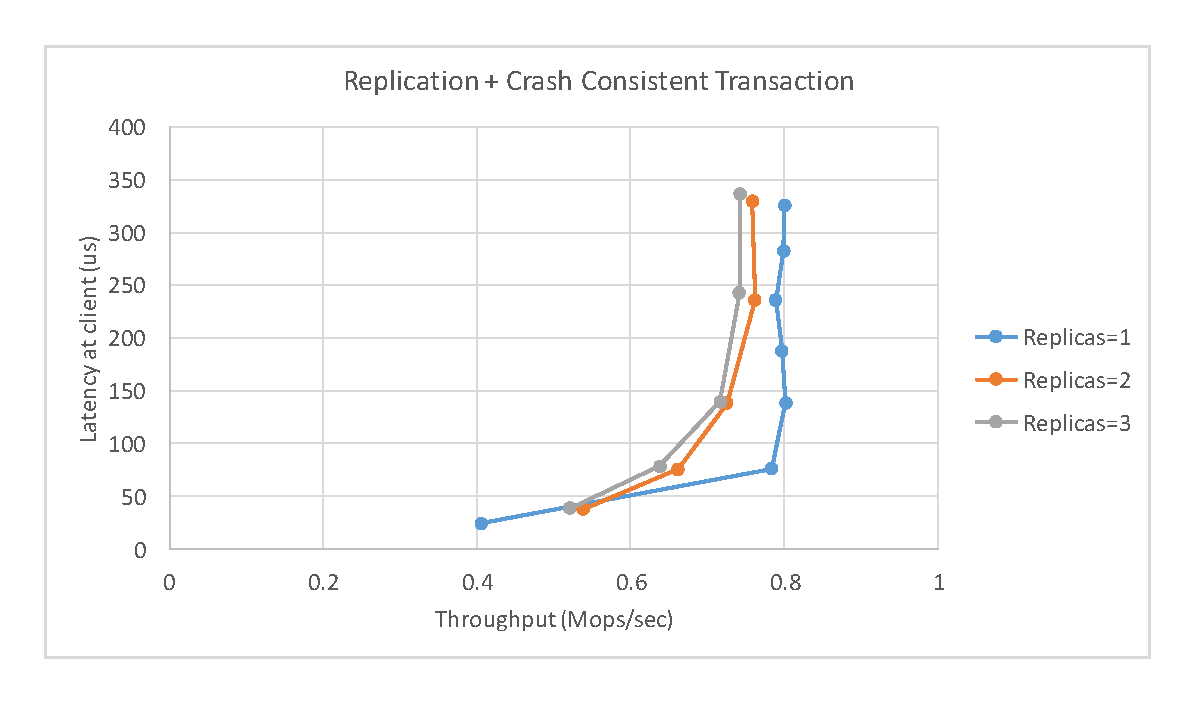
\includegraphics[width=\textwidth,height=3cm]{results/cc_mops.pdf}
  \caption{Crash Consistency}
  \label{fig:cc_rep}
\end{minipage} &
  \hspace{-0.37in}
\begin{minipage}{0.25\textwidth}
  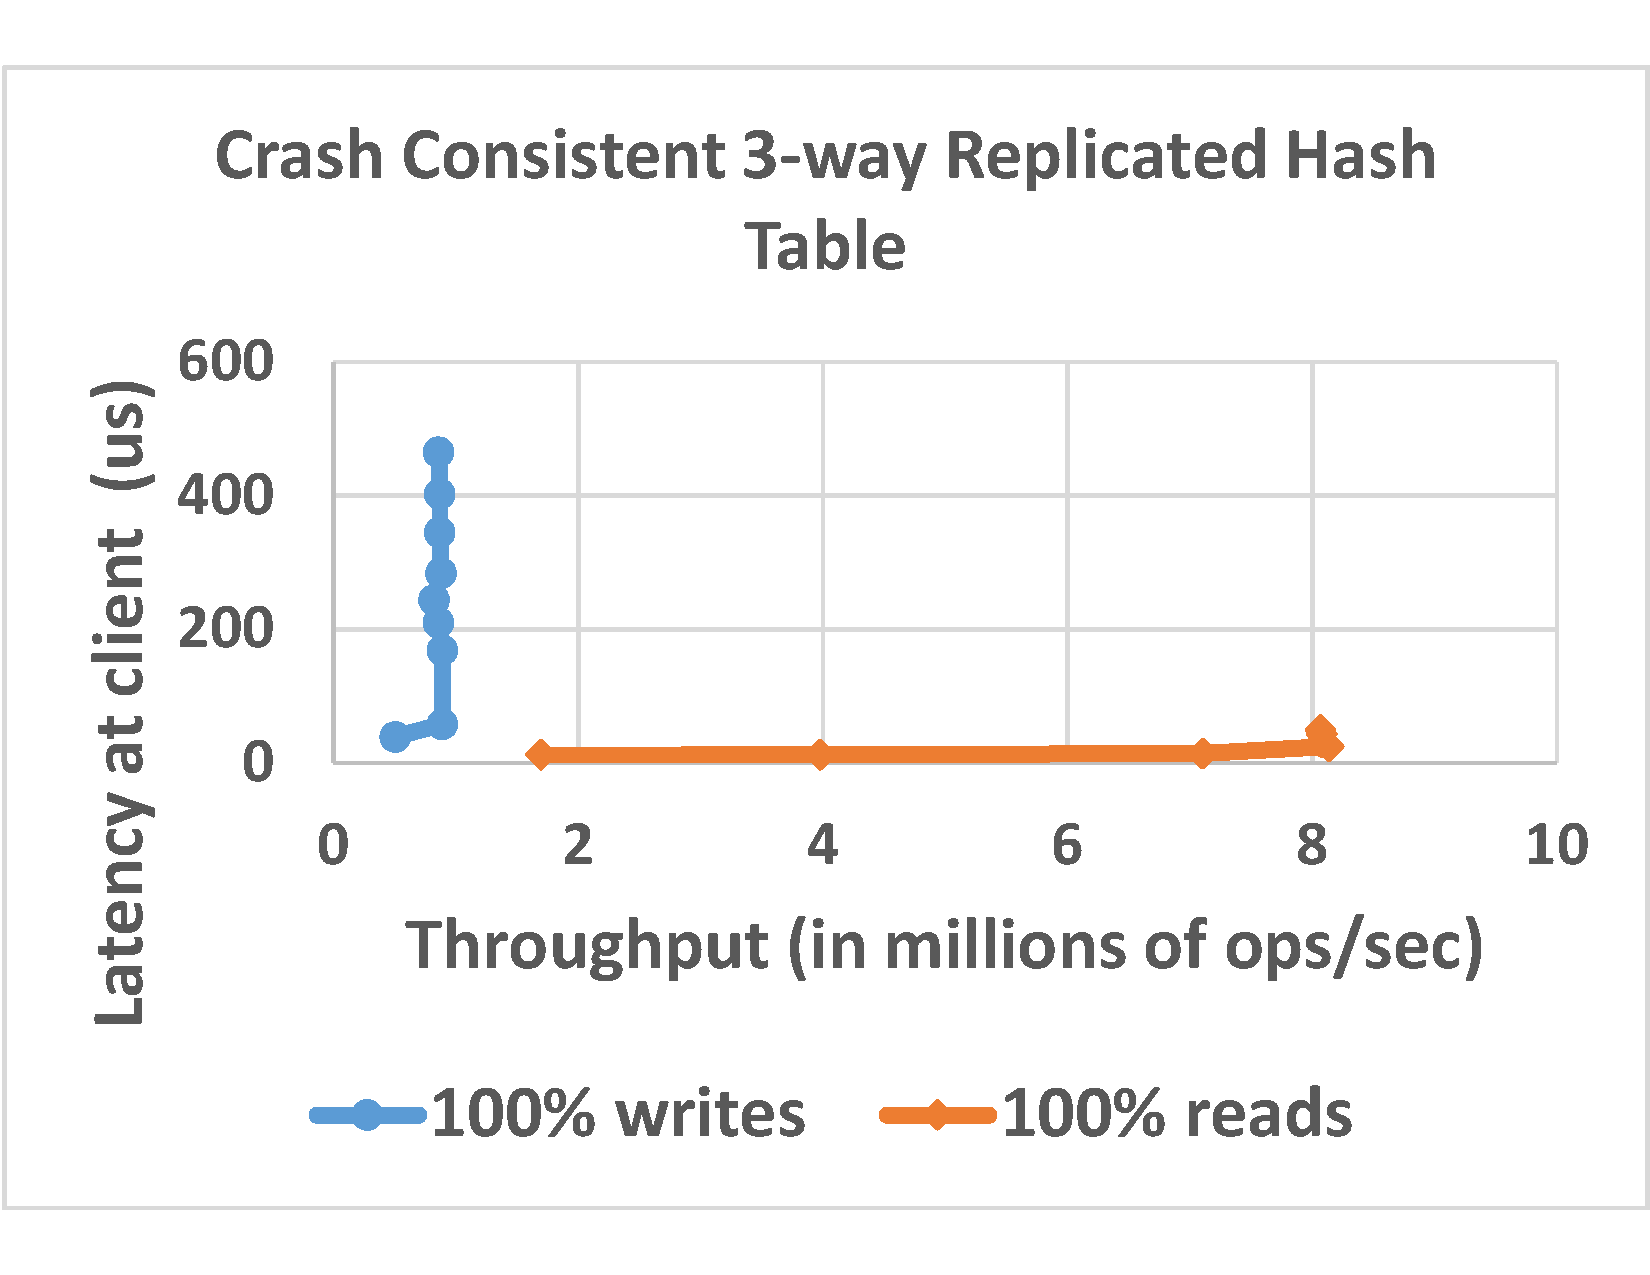
\includegraphics[width=\textwidth,height=3cm]{results/app_mops.pdf}
  \caption{Hash Table}
  \label{fig:app_rep}
\end{minipage}
\end{tabular}
\end{figure}

\section{Conclusion}
Cyclone allows developers to add availability to applications built on top of
libraries such as NVML and achieve good performance on commodity networking
hardware. A key question is whether Cyclone can be used for other applications
such as filesystems ? We believe that the requirement for scaling across
multiple replication quorums can be satisfied by applications where the scalable
commutativity rule~\cite{scalable_commutativity} applies to common case
primitives. Although our intitial release of Cyclone will be for
key value style applications, our future research is based on this hypothesis.
\newcommand\myurl[2]{\url{#1}}
\bibliographystyle{acm}
\bibliography{paper}

\end{document}



